\documentclass[tikz]{standalone}
\usepackage{standalone}
\usepackage{pgf,tikz,physics}
\usepackage{mathrsfs}
\usetikzlibrary{arrows}
\begin{document}
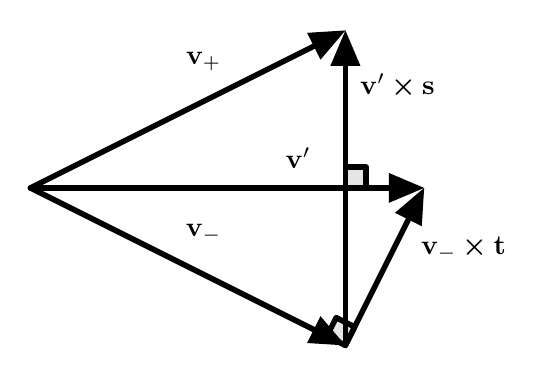
\begin{tikzpicture}[line cap=round,line join=round,>=triangle 45,x=1cm,y=1cm]
\draw[line width=2pt,fill=black,fill opacity=0.10000000149011612] (4.117544391373898,-1.7649112172522041) -- (3.882455608626102,-1.647366825878306) -- (3.764911217252204,-1.882455608626102) -- (4,-2) -- cycle;
\draw[line width=2pt,fill=black,fill opacity=0.10000000149011612] (4.262837249485876,0) -- (4.262837249485876,0.2628372494858757) -- (4,0.2628372494858757) -- (4,0) -- cycle;
\draw [->,line width=2pt] (0,0) -- (4,-2);
\draw [->,line width=2pt] (0,0) -- (4,2);
\draw [->,line width=2pt] (4,-2) -- (4,2);
\draw [->,line width=2pt] (0,0) -- (5,0);
\draw [->,line width=2pt] (4,-2) -- (5,0);
\draw[color=black] (2.20,-0.58) node {$\vb{v}_-$};
\draw[color=black] (2.20,1.61) node {$\vb{v}_+$};
\draw[color=black] (4.66,1.29) node {$\vb{v}' \cp \vb{s}$};
\draw[color=black] (3.40,0.38) node {$\vb{v}'$};
\draw[color=black] (5.50,-0.77) node {$\vb{v}_- \cp \vb{t}$};
\end{tikzpicture}
\end{document}
